\section{Detection}
The sliding windows algorithm has been implemented as described in the project
description.
The samples from this algorithm can be assessed by the trained classifier,
as long as the number of features in each processed window is the same as the classifier was trained on.

To test the detection we took a photo of a sheet of paper with some text and drawings.
The sheet has text of two different sizes, as well as some drawings of non-text.
The edges of the sheet, as well as of the table the sheet lies upon.
The window size of the sliding window algorithm is fitted to the larger text.
Running the classifier on the windows, we can visualise the results by selecting the windows where the confidence of the classifier is above a specific threshold, and draw an indicator on top of the photo.
An example of this can be seen in Figure \ref{fig:illuminati}.
As we can see, the detector does higlight where there is text to some degree,
but it is also tripped up by the drawings and somee edges in the "background".

\begin{figure}[H]
    \centering
    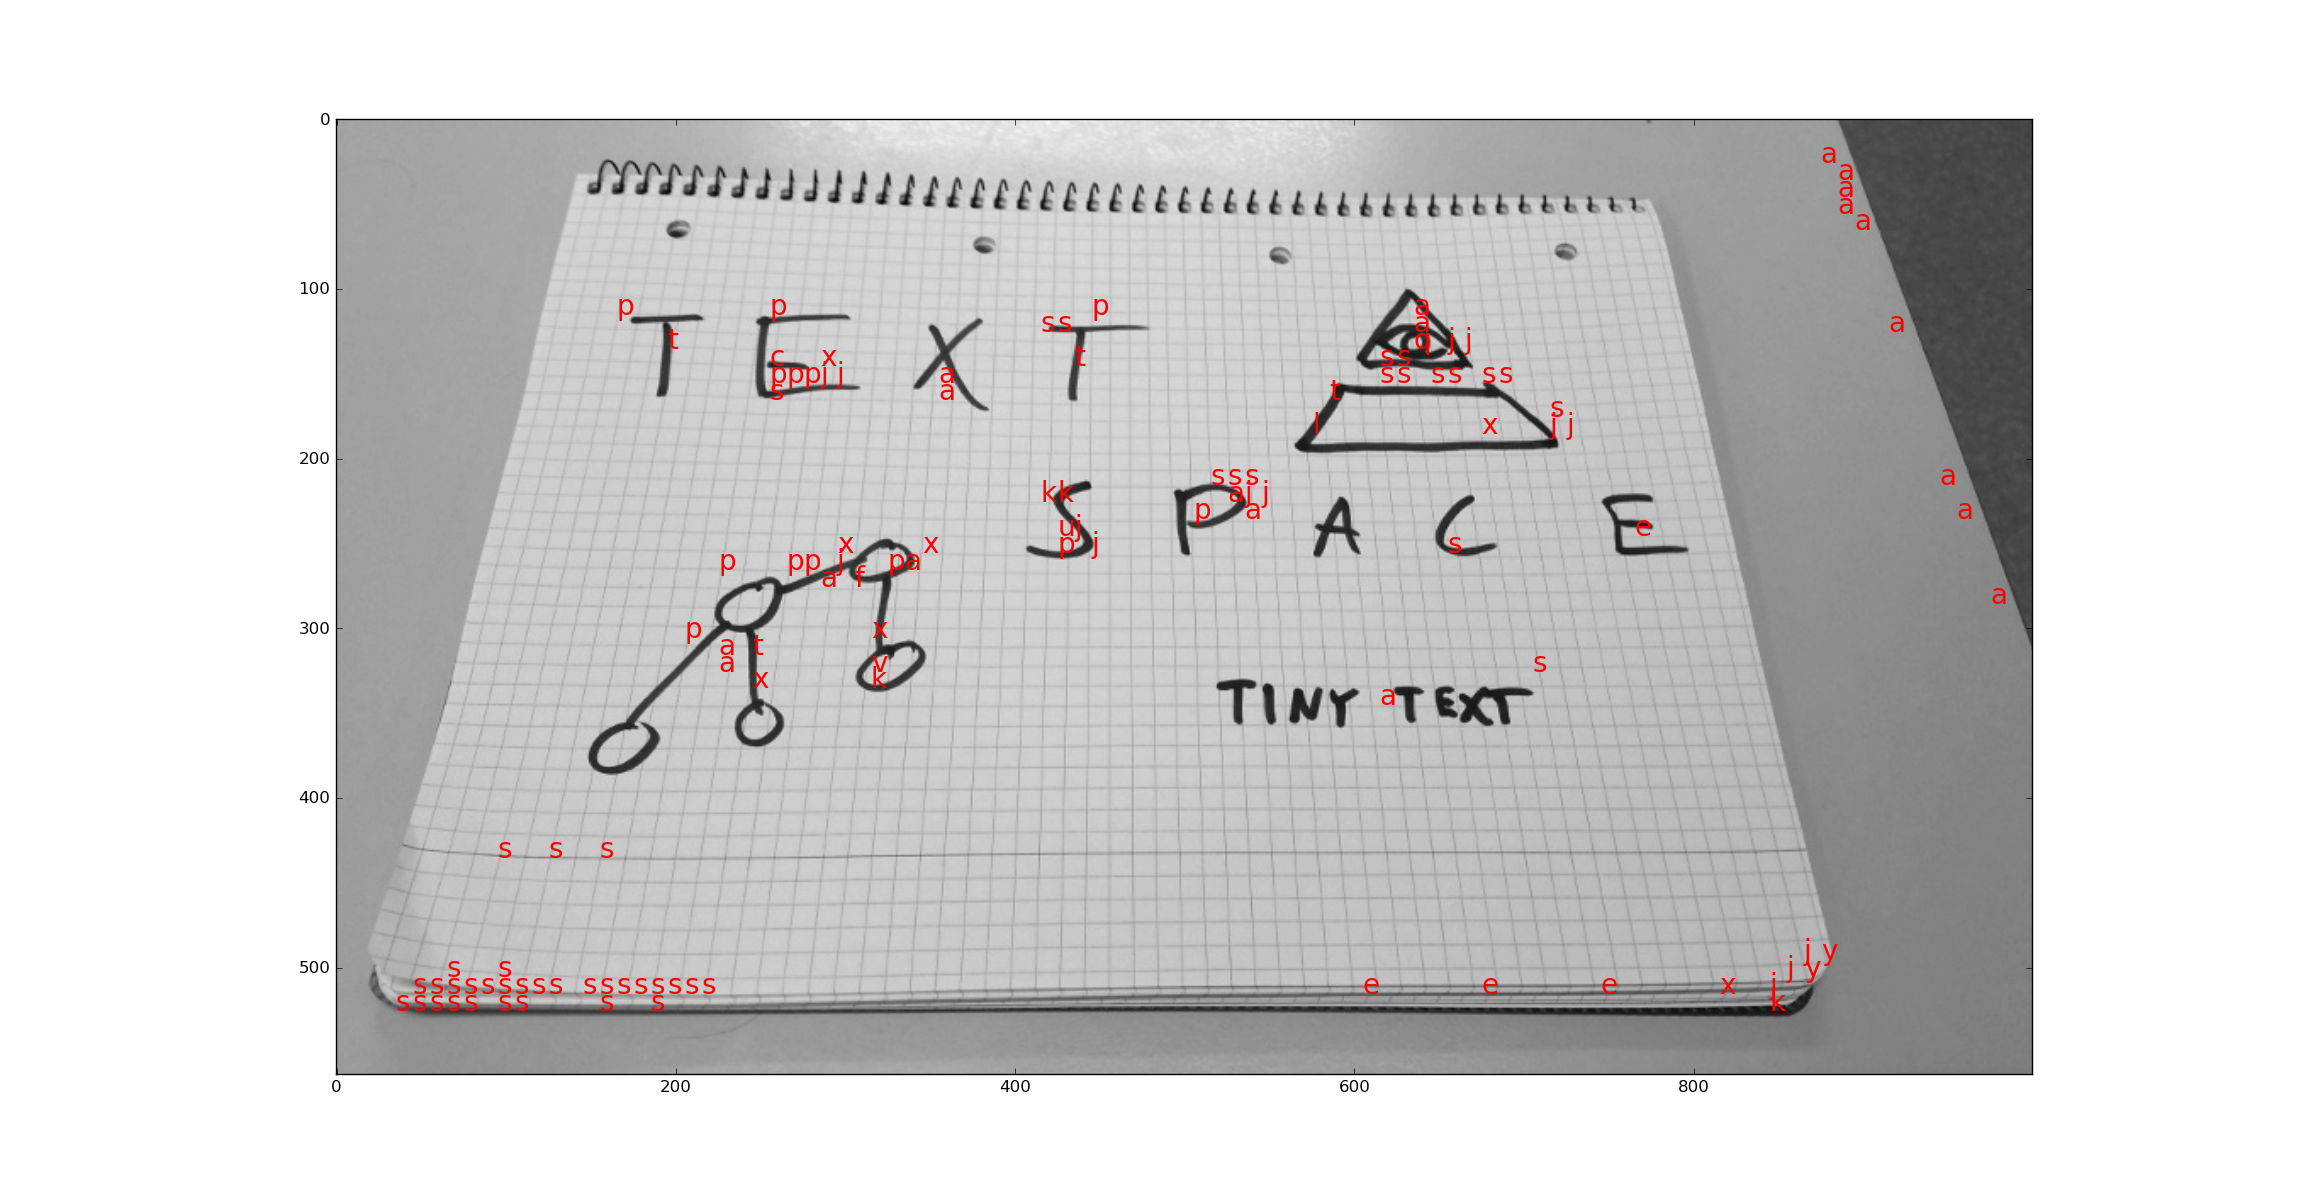
\includegraphics[width=\linewidth]{img/illuminati}
    \caption{Detection results.}
    \label{fig:illuminati}
\end{figure}

We tried different methods and parameters for this experiment.
The best results are seen in Figure \ref{fig:illuminati},
with the relevant parameters shown in Table \ref{tbl:illuminati}.

\begin{table}[H]
    \centering
    \begin{tabular}{l|l}
        Preprocessing   &   \texttt{oriented\_gradients}    \\\hline
        Classifier      &   \texttt{LinearSVC}              \\\hline
        Threshold       &   $0.5$
    \end{tabular}
    \caption{Parameters for experiment seen in Figure \ref{fig:illuminati}}.
    \label{tbl:illuminati}
\end{table}

This experiment has been stored to the file \texttt{experiment\_detection\_photo\_hog\_svc.py} and can be recreated by running it.

An interesting observation at this stage is how adding the binarization preprocessing before the HOG preprocessing changes the outcome.
This increases the number of false positives drastically around the edges of the paper in the photo.
The binarization is accentuating the edges and this creating something which looks like letters to the classifier.
Looking closer at what letters the classifier thinks it is seeing near the edges, we see things like "i" and "l", which supports this assumption.

